% LaTeX source for textbook ``ThinkCPP , a game perspective''
% Copyright (C) 2023  Lisa Patacchiola


\chapter{Integrated Development Environments}
C++ has standards so code should work in different compilers. But, the 
environments that can compile and run your code can be different. Here
are some descriptions on how to use some of the popular development
environments. This appendix has information on Replit and Visual Studio Code.
\section{Installing}
\label{installide}
Before you use a compiler, there is usually some setup. Some need to
be installed on your computer. Others need an account to be created.
Here are the steps to get your compiler ready to be used.
\subsection{Replit}
Replit does not need to be installed. It is an online coding environment.
This IDE will work well for those using a Chrome book. The one thing that you will need to do is go to \url{http://replit.com} and create an 
account there.
\subsection{Visual Studio Code}
There are many steps to get C++ to work with Visual Studio code. Visual Studio Code works in Windows, macOS and Linux. First,
download and install the tool. The tool is available at this 
website: \url{https://code.visualstudio.com/}. Click the appropriate
down button for your computer.

Once it is installed, you will need to install the C/C++ extension for VS Code. You can install the C/C++ extension by searching for 'c++' in the Extensions view (Ctrl+Shift+X).

The next steps are to get it working with the Microsoft compiler.
If you have a recent version of the compiler installed, you can use the tools and you are done with the installation. If not, you will need to do the following:

Go online to the Visual Studio Downloads page. On that page, scroll
down until you see {\tt Tools for Visual Studio} under the All Downloads section and click the download button for "Build Tools for Visual Studio 2022".

This will download and launch the Visual Studio Installer, which will bring up a dialog showing the available Visual Studio Build Tools workloads. Check the Desktop development with C++ workload and select Install. Once it is done, you should be ready to create a project.

For more information, check this page:
\url{https://code.visualstudio.com/docs/cpp/config-msvc }

\section{Setting up a project}
\label{setupproject}
Want to code on your own? This section will some helpful instructions on
how to start coding with some common coding environments.
\subsection{Replit}
Once you log in to you account, you should be able to see the full
menu. Look for the "Create" button that is on the top left. The button
should look like figure \ref{fig:createreplit}:
\begin{figure}[h]
    \centering
    
\includegraphics{images/CreateButtonReplit.PNG}
    \caption{The Create button for Replit}
    \label{fig:createreplit}
\end{figure}
Once you click that button, another menu will open. Here you will have a chance to choose the language
that you will be using. Click on the area under the "Template" in the left top section of the menu. Look for the C++ template. Once the template is chosen, click on the "Title" area and choose a name 
for your project. If you have the template and the name, the next step 
is to click the "Create Repl" button. Soon after, you will be in the
development environment.
\begin{figure}[h]
    \centering
    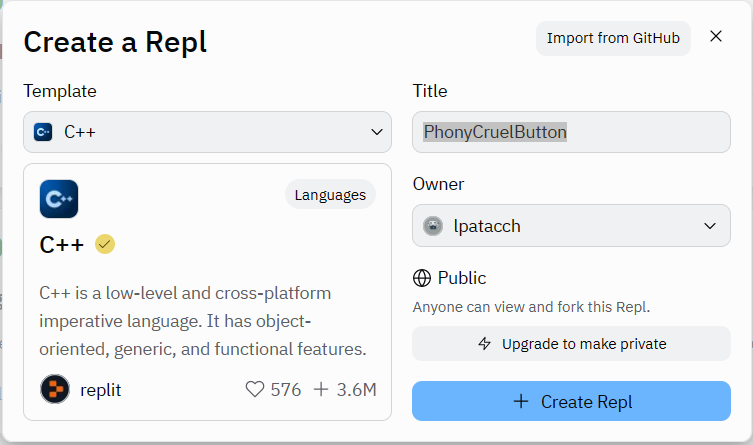
\includegraphics[width = 10cm]{images/createreplitmenu.PNG}
    \caption{Template and Naming your Replit}
    \label{fig:replitmenu}
\end{figure}


For more information, there is the documentation from replit which explains the startup in more detail. 
\url{https://docs.replit.com/programming-ide/introduction-to-the-workspace}
\subsection{Visual Studio Code}
First, run the "Developer Command Prompt for Visual Studio". That will open up a command line. From there, go to the area where you want your project to be. Then, make the directory (mkdir), go into the directory (cd) and run visual studio code from that location (code). For example, if you want a "newproj" project.

\begin{verbatim}
mkdir newproj
cd newproj
code .    
\end{verbatim}

Visual Studio Code will now be running. You can click the "new file" button and it will add a file to your project.

\section{Settings}
Most Integrated Development Environments work well as soon as you install them. They are designed so you do not have to worry about all the various options the compiler and linker can use. This section will explain options you may want to set on your IDE to help you code. NOTE: Your IDE will work fine without these changes. They are the ones that I have found particularly helpful.
\subsection{Replit}
\index{replit}
\subsubsection{Turning on warnings}
\index{warnings}
\label{showwarning}
One particular feature I like to use is to "show all warnings". If you remember, warnings are a way that the compiler can show you that it noticed some code that could be an error. The code does not have a problem with it's syntax, but many times code in this pattern is a logic error.

For example, this code compiles without an error on Replit:
\begin{lstlisting}
  if (x=0)          \\ There is only 1 equal sign
  {
    std::cout<<"woo";
  }
\end{lstlisting}
It only has one equal sign, so instead of comparing the variable
to zero, it set the variable to zero. Technically, that code does not have a syntax problem. But, very few people would want to set a value here. They were expecting the code to compare values.

Luckily, you can set options in the Replit environment to let you know that there could be a mistake.

To make your environment less cluttered, Replit hides the configuration files as a default. But, you can show these files so you can edit them. First, click the three dots next to the word "Files" on the left. That should open a menu with an option to "Show hidden files". Click that option. The menu should look like Figure \ref{fig:ShowHiddenMenu}

\begin{figure}[h]
    \centering
    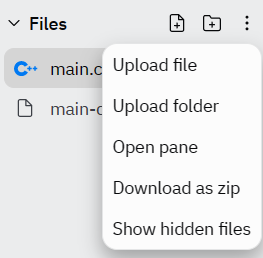
\includegraphics{images/showhidden.PNG}
    \caption{The Menu that Displays when you press the three Dots}
    \label{fig:ShowHiddenMenu}
\end{figure}

The file that you will be editing is called "Makefile". This file holds the special options that are used when compiling and linking. Look for a line in the file matches this:

\begin{verbatim}
    override CXXFLAGS += -g -Wno-everything    
\end{verbatim}

The -Wno-everything flag is telling the compiler to ignore all warnings. That is not what we want. Instead, change that line to:

\begin{verbatim}
    override CXXFLAGS += -g -Weverything
\end{verbatim}

Instead of hiding all the warnings, it will show them instead. There are other flags that do not show as many warnings, but I prefer to see all the possible problems with my code.

\subsubsection{Using a certain version of the C++ standard}
\label{changestandard}
Although Replit does compile C++ code, it defaults to an older version of the language. C++ has continually added new features as the years have gone on. For example, smart pointers were not added to the language until 2011.

At the time of the writing of this book, the default version of C++ that Replit uses is the 2014 standard. If you want to use some of the newer features, you need to tell it to use a different version of the standard. That is achievable by changing the Makefile again. Look for the same overide CXXFLAGS line that you changed in the last section. Change that line to the following line:

\begin{verbatim}
override CXXFLAGS += -g -std=c++20 -Weverything -Wno-c++98-compat
\end{verbatim}

The important part is the {\tt -std=} part of the line. That is telling the compiler what standard to use. c++20 is telling it to use the 2020 version of the standard. I also added the {\tt -Wnoc++98-compat"} to the line. That shuts off any warnings complaining that the code is not compatible with the 1998 version of C++. That isn't necessary to get the 2020 version to run, but I found it helpful to remove the warnings that were no longer pertinent. If I am using the 2020 version of the standard because I want to use the new language features, I am not worried about if my code works with a 1998 version of the compiler.

\subsection{Visual Studio Code}
At the time of the writing of this book, Visual Studio Code defaults to C++14, If you want to use any of the newer features, you need to tell
the compiler. To turn on the different standard, open the tasks.json file. There will be a section listed as: "args". Put the following in the list of items in that section.
\begin{verbatim}
"/std:c++20",    
\end{verbatim}
That should turn on the C++20 standard. If you want the latest that is
available, you can use this instead:
\begin{verbatim}
"/std:c++latest",
\end{verbatim}
to use the most recent version.

That will change the way the tool compiles, but it will not change the IntelliSense (this is what makes the red squiggles underneath errors). That setting is found in the c\_cpp\_properties.json file. If your project does not have that yet, Visual Studio Code can make one for you. First, type Ctrl-Shft-P to get the menu. Then, choose C/C++: Edit Configurations (UI). That will open up a C/C++ Configurations menu. Scroll down until you get to the "C++ standard" section. From there, you can change it to whatever standard you want. The code in this book has been tested with the C++23 Intellisense.

